\documentclass[a4paper, 12pt]{article}
\usepackage{titling}
\usepackage{array}
\usepackage{booktabs}
\usepackage{enumitem}
\usepackage{graphicx}
\usepackage{hyperref}
\usepackage{amssymb}


\usepackage{listings}
\setlength{\heavyrulewidth}{1.5pt}
\setlength{\abovetopsep}{4pt}
\setlength{\parindent}{0pt}
\graphicspath{{.}}

\usepackage[margin=1in]{geometry}

% Must be after geometry
\usepackage{fancyhdr}
\pagestyle{fancy}
\fancyhf{}
\rhead{SEE Assignment 1}
\lhead{P.Lukin, E. Ovchinnikova}
\cfoot{\thepage}

\setlength{\droptitle}{-5em}

\title{Scientific Experimentation and Evaluation  \\
				Assignment: 1.2}
\author{Petr Lukin, Evgeniya Ovchinnikova}
\date{Lecture date: $04^{th}$ October 2016}

\begin{document}



\maketitle

\section{Experiments}

Our task was to run 5 experiments each repeated at least 20 times. We ran the following experiments: forward motion, 90$^{\circ}$ arc motion to the left, 90$^{\circ}$ arc motion to the right, 30$^{\circ}$ arc motion to the left and 30$^{\circ}$ arc motion to the right.\\
While experimenting we have realized the necessity of modifying code for 90$^{\circ}$ arc left and right motion so the robot trajectory would fit a for paper size. Moreover, to improve the process of adjustment of the robot's position on the paper. Before we had a function that makes robot to wait for a certain time before it starts moving the motors, so we could have time to adjust it to the "garage" position. Now this function is replaced with a function for waiting for a button pressing. That allows to regulate the time we need to install the robot. The modified Java code for forward motion, 90$^{\circ}$ arc motion to the left, 90$^{\circ}$ arc motion to the right, 30$^{\circ}$ arc motion to the left and 30$^{\circ}$ arc motion to the right is shown below:

\begin{lstlisting}
package LegoNXT;

import lejos.nxt.LightSensor;
import lejos.nxt.Motor;
import lejos.nxt.SensorPort;
import lejos.robotics.navigation.DifferentialPilot;
import lejos.robotics.navigation.MoveController;
import lejos.util.Delay;
import lejos.nxt.Button;

public class goStraight {

	public static void main(String[] args) {
		double arcRad = 40;
		double angle = 90;
		double arcLen = Math.PI*2*arcRad*angle/360;
		double trackWidth = 12;
		Button.LEFT.waitForPressAndRelease();
		LightSensor lightSens1 = new LightSensor(SensorPort.S1);
		LightSensor lightSens2 = new LightSensor(SensorPort.S2);
		DifferentialPilot dp = new DifferentialPilot(
		MoveController.WHEEL_SIZE_NXT1, trackWidth, Motor.B,
		Motor.C, true);
		lightSens1.setHigh(100);
		lightSens2.setHigh(100);
		Button.RIGHT.waitForPressAndRelease();
		dp.setTravelSpeed(10);
		dp.travel(-arcLen);
		dp.stop();
		Button.ESCAPE.waitForPressAndRelease();
	}
}

***

package LegoNXT;

import lejos.nxt.Motor;
import lejos.nxt.SensorPort;
import lejos.robotics.navigation.DifferentialPilot;
import lejos.robotics.navigation.MoveController;
import lejos.util.Delay;
import lejos.nxt.LightSensor;
import lejos.nxt.Button;

public class goLeft {

	public static void main(String[] args) {
		double arcRad = 25;
		double angle = 90;
		double trackWidth = 12;
		Button.LEFT.waitForPressAndRelease();
		LightSensor lightSens1 = new LightSensor(SensorPort.S1);
		LightSensor lightSens2 = new LightSensor(SensorPort.S2);
		DifferentialPilot dp = new DifferentialPilot(
		MoveController.WHEEL_SIZE_NXT1, trackWidth, Motor.B,
		Motor.C, true);
		lightSens1.setHigh(100);
		lightSens2.setHigh(100);
		Button.RIGHT.waitForPressAndRelease();
		dp.setTravelSpeed(10);
		dp.arc(-arcRad, angle);
		dp.stop();
		Button.ESCAPE.waitForPressAndRelease();
	}
}

***

package LegoNXT;

import lejos.nxt.LightSensor;
import lejos.nxt.Motor;
import lejos.nxt.SensorPort;
import lejos.robotics.navigation.DifferentialPilot;
import lejos.robotics.navigation.MoveController;
import lejos.util.Delay;
import lejos.nxt.Button;

public class goRight {

	public static void main(String[] args) {
		double arcRad = 25;
		double angle = 90;
		double trackWidth = 12;
		Button.LEFT.waitForPressAndRelease();
		LightSensor lightSens1 = new LightSensor(SensorPort.S1);
		LightSensor lightSens2 = new LightSensor(SensorPort.S2);
		DifferentialPilot dp = new DifferentialPilot(
		MoveController.WHEEL_SIZE_NXT1, trackWidth, Motor.B,
		Motor.C, true);
		lightSens1.setHigh(100);
		lightSens2.setHigh(100);
		Button.RIGHT.waitForPressAndRelease();
		dp.setTravelSpeed(10);
		dp.arc(arcRad, -angle);
		dp.stop();
		Button.ESCAPE.waitForPressAndRelease();
	}
}

***
package LegoNXT;

import lejos.nxt.Button;
import lejos.nxt.LightSensor;
import lejos.nxt.Motor;
import lejos.nxt.SensorPort;
import lejos.robotics.navigation.DifferentialPilot;
import lejos.robotics.navigation.MoveController;

public class goSlightlyLeft {
	public static void main(String[] args) {
		double arcRad = 120;
		double angle = 30;
		double trackWidth = 12;
		Button.LEFT.waitForPressAndRelease();
		LightSensor lightSens1 = new LightSensor(SensorPort.S1);
		LightSensor lightSens2 = new LightSensor(SensorPort.S2);
		DifferentialPilot dp = new DifferentialPilot(
		MoveController.WHEEL_SIZE_NXT1, trackWidth, Motor.B,
		Motor.C, true);
		lightSens1.setHigh(100);
		lightSens2.setHigh(100);
		Button.RIGHT.waitForPressAndRelease();
		dp.setTravelSpeed(10);
		dp.arc(-arcRad, angle);
		dp.stop();
		Button.ESCAPE.waitForPressAndRelease();
	}
}
***
package LegoNXT;

import lejos.nxt.Motor;
import lejos.nxt.SensorPort;
import lejos.robotics.navigation.DifferentialPilot;
import lejos.robotics.navigation.MoveController;
import lejos.util.Delay;
import lejos.nxt.LightSensor;
import lejos.nxt.Button;

public class goSlightlyRight {

	public static void main(String[] args) {
		double arcRad = 120;
		double angle = 30;
		double trackWidth = 12;
		Button.LEFT.waitForPressAndRelease();
		LightSensor lightSens1 = new LightSensor(SensorPort.S1);
		LightSensor lightSens2 = new LightSensor(SensorPort.S2);
		DifferentialPilot dp = new DifferentialPilot(
		MoveController.WHEEL_SIZE_NXT1, trackWidth, Motor.B,
		Motor.C, true);
		lightSens1.setHigh(100);
		lightSens2.setHigh(100);
		Button.RIGHT.waitForPressAndRelease();
		dp.setTravelSpeed(10);
		dp.arc(arcRad, -angle);
		dp.stop();
		Button.ESCAPE.waitForPressAndRelease();
	}
}

\end{lstlisting}	

For the experiment we used a setup described in section "4 What and how we are planning to do" of assignment 1.1with updated program code. The robot was placed on a large marked paper (Fig.\ref{fig:paper}) to a "garage" position (Fig.\ref{fig:garage}) and launched 105 times to five different directions.

\begin{figure}[h]
  \centering
  \caption{Paper with the "garage" marks.\label{fig:paper}}
  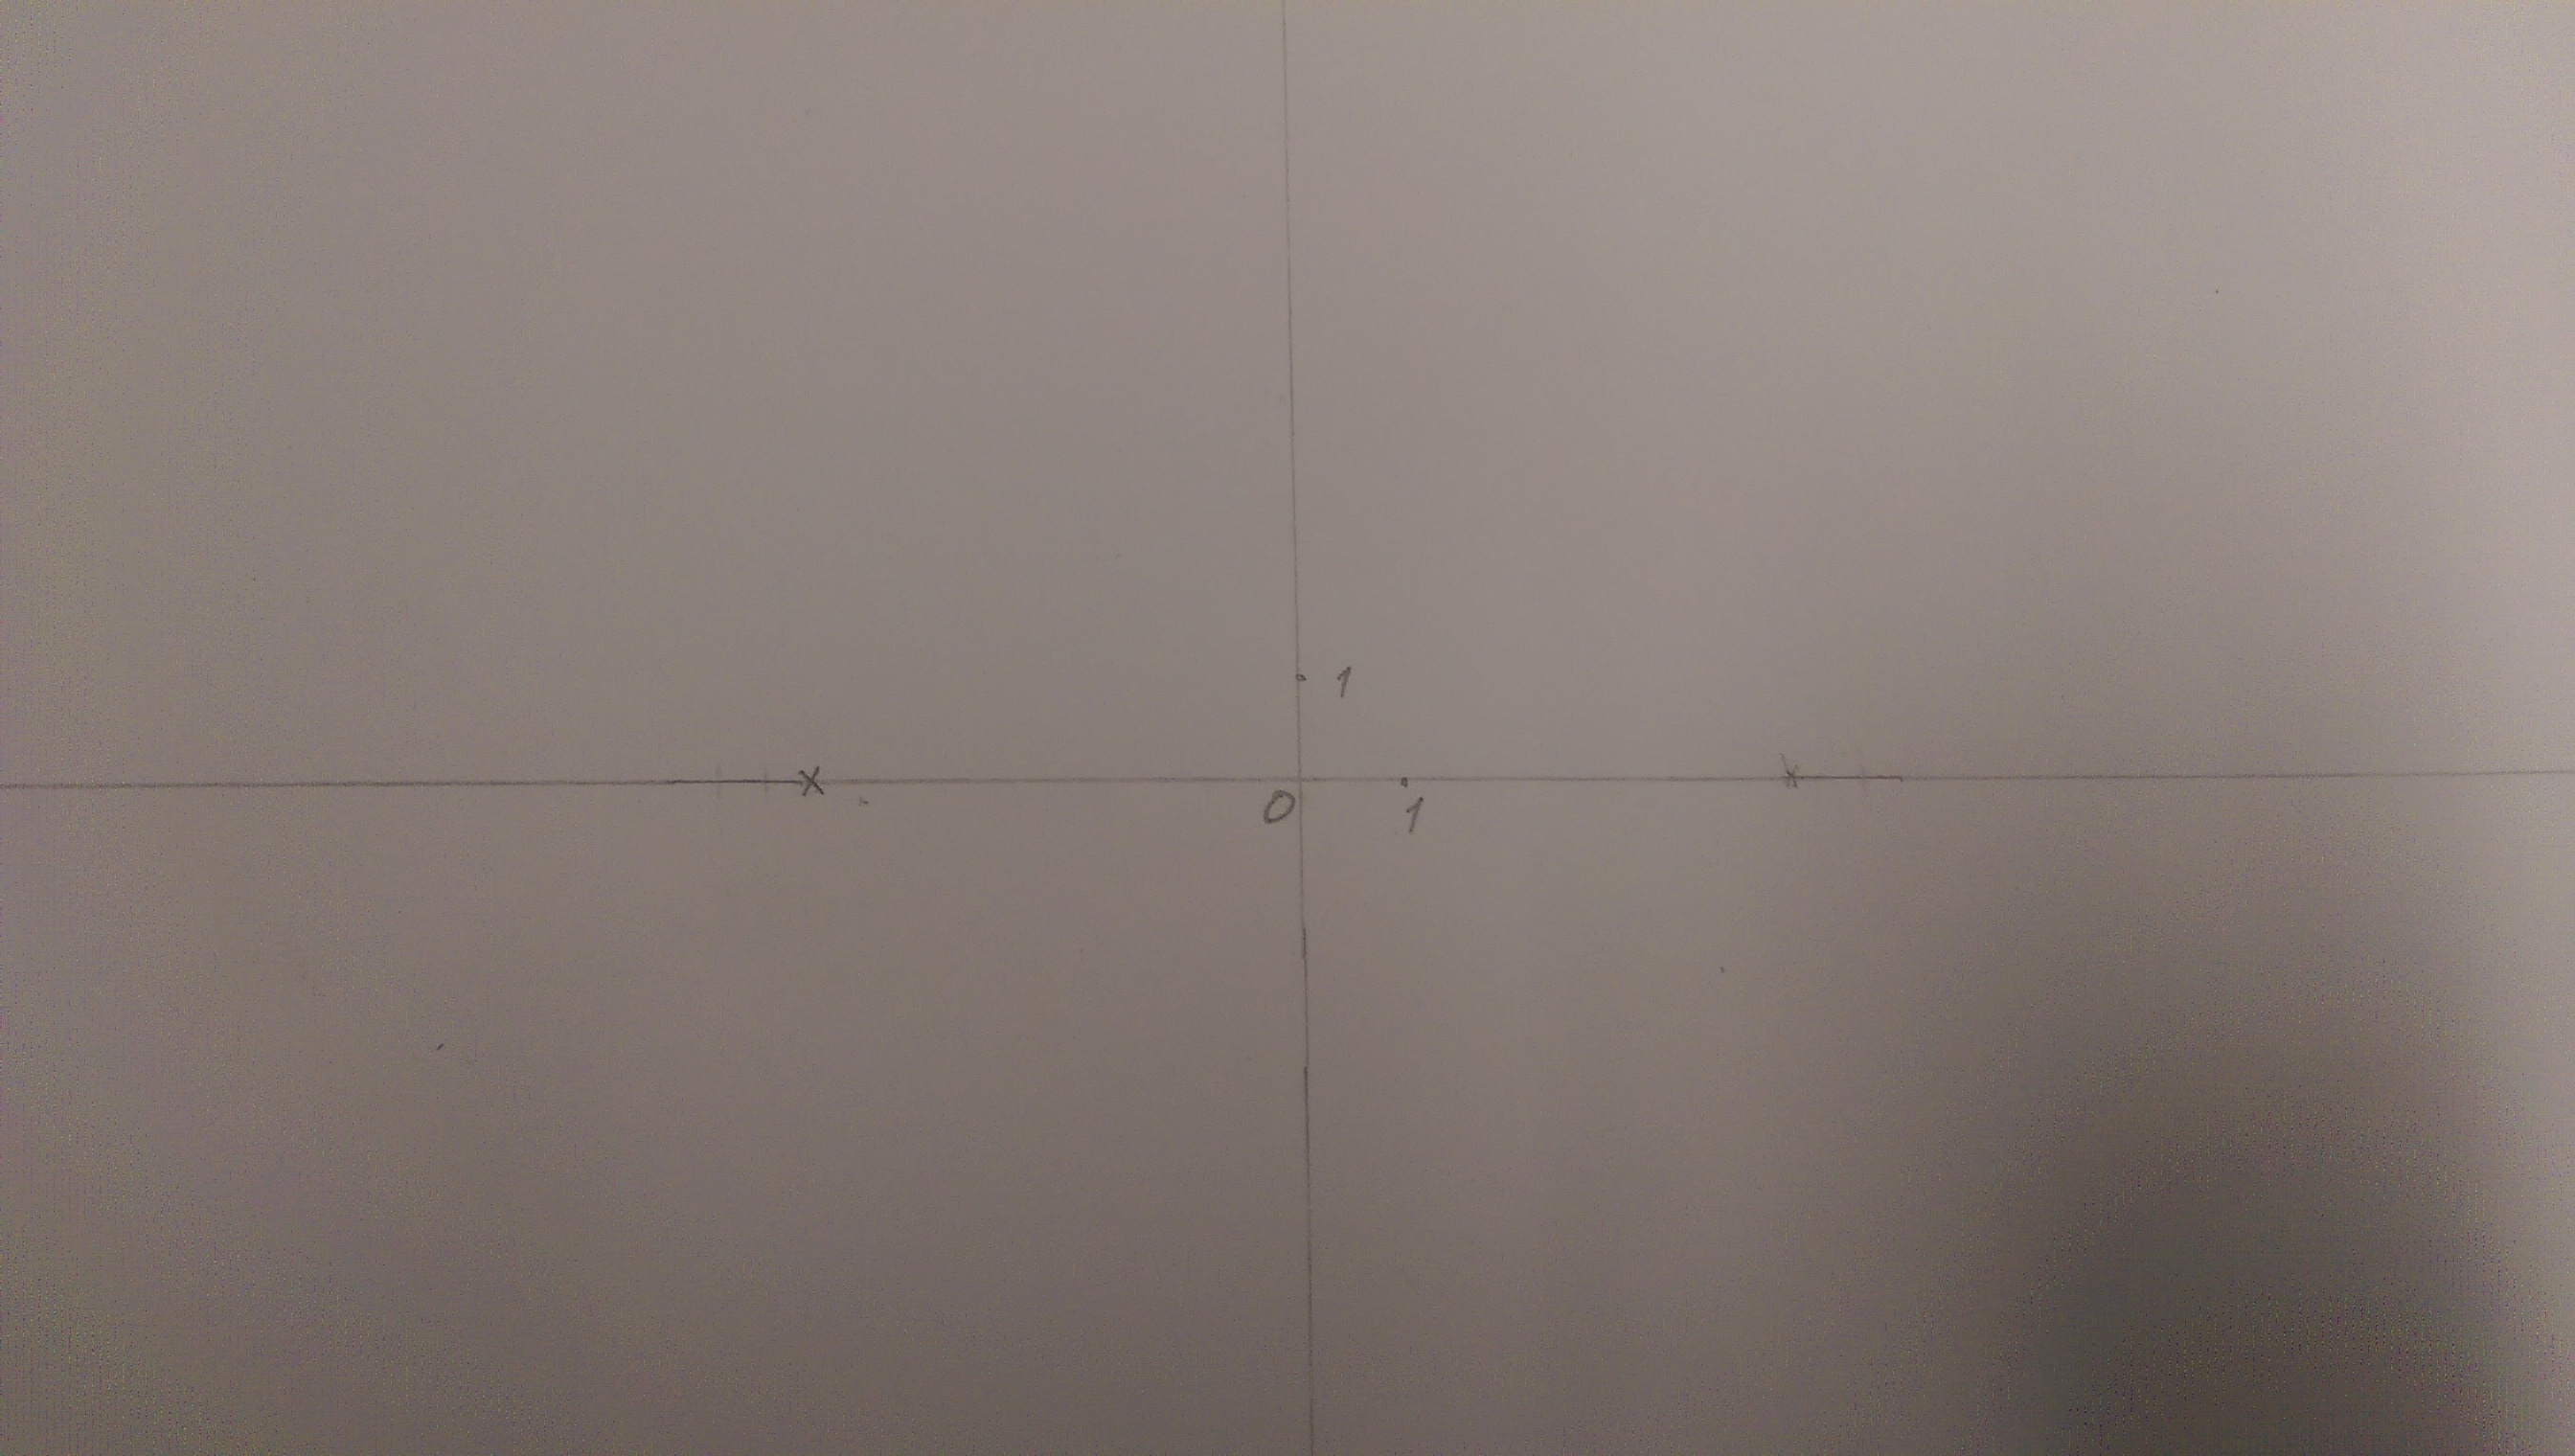
\includegraphics[width=0.8\textwidth]{markedPaper}
\end{figure}

\begin{figure}[h]
  \centering
  \caption{Robot placed into the "garage" position.\label{fig:garage}}
  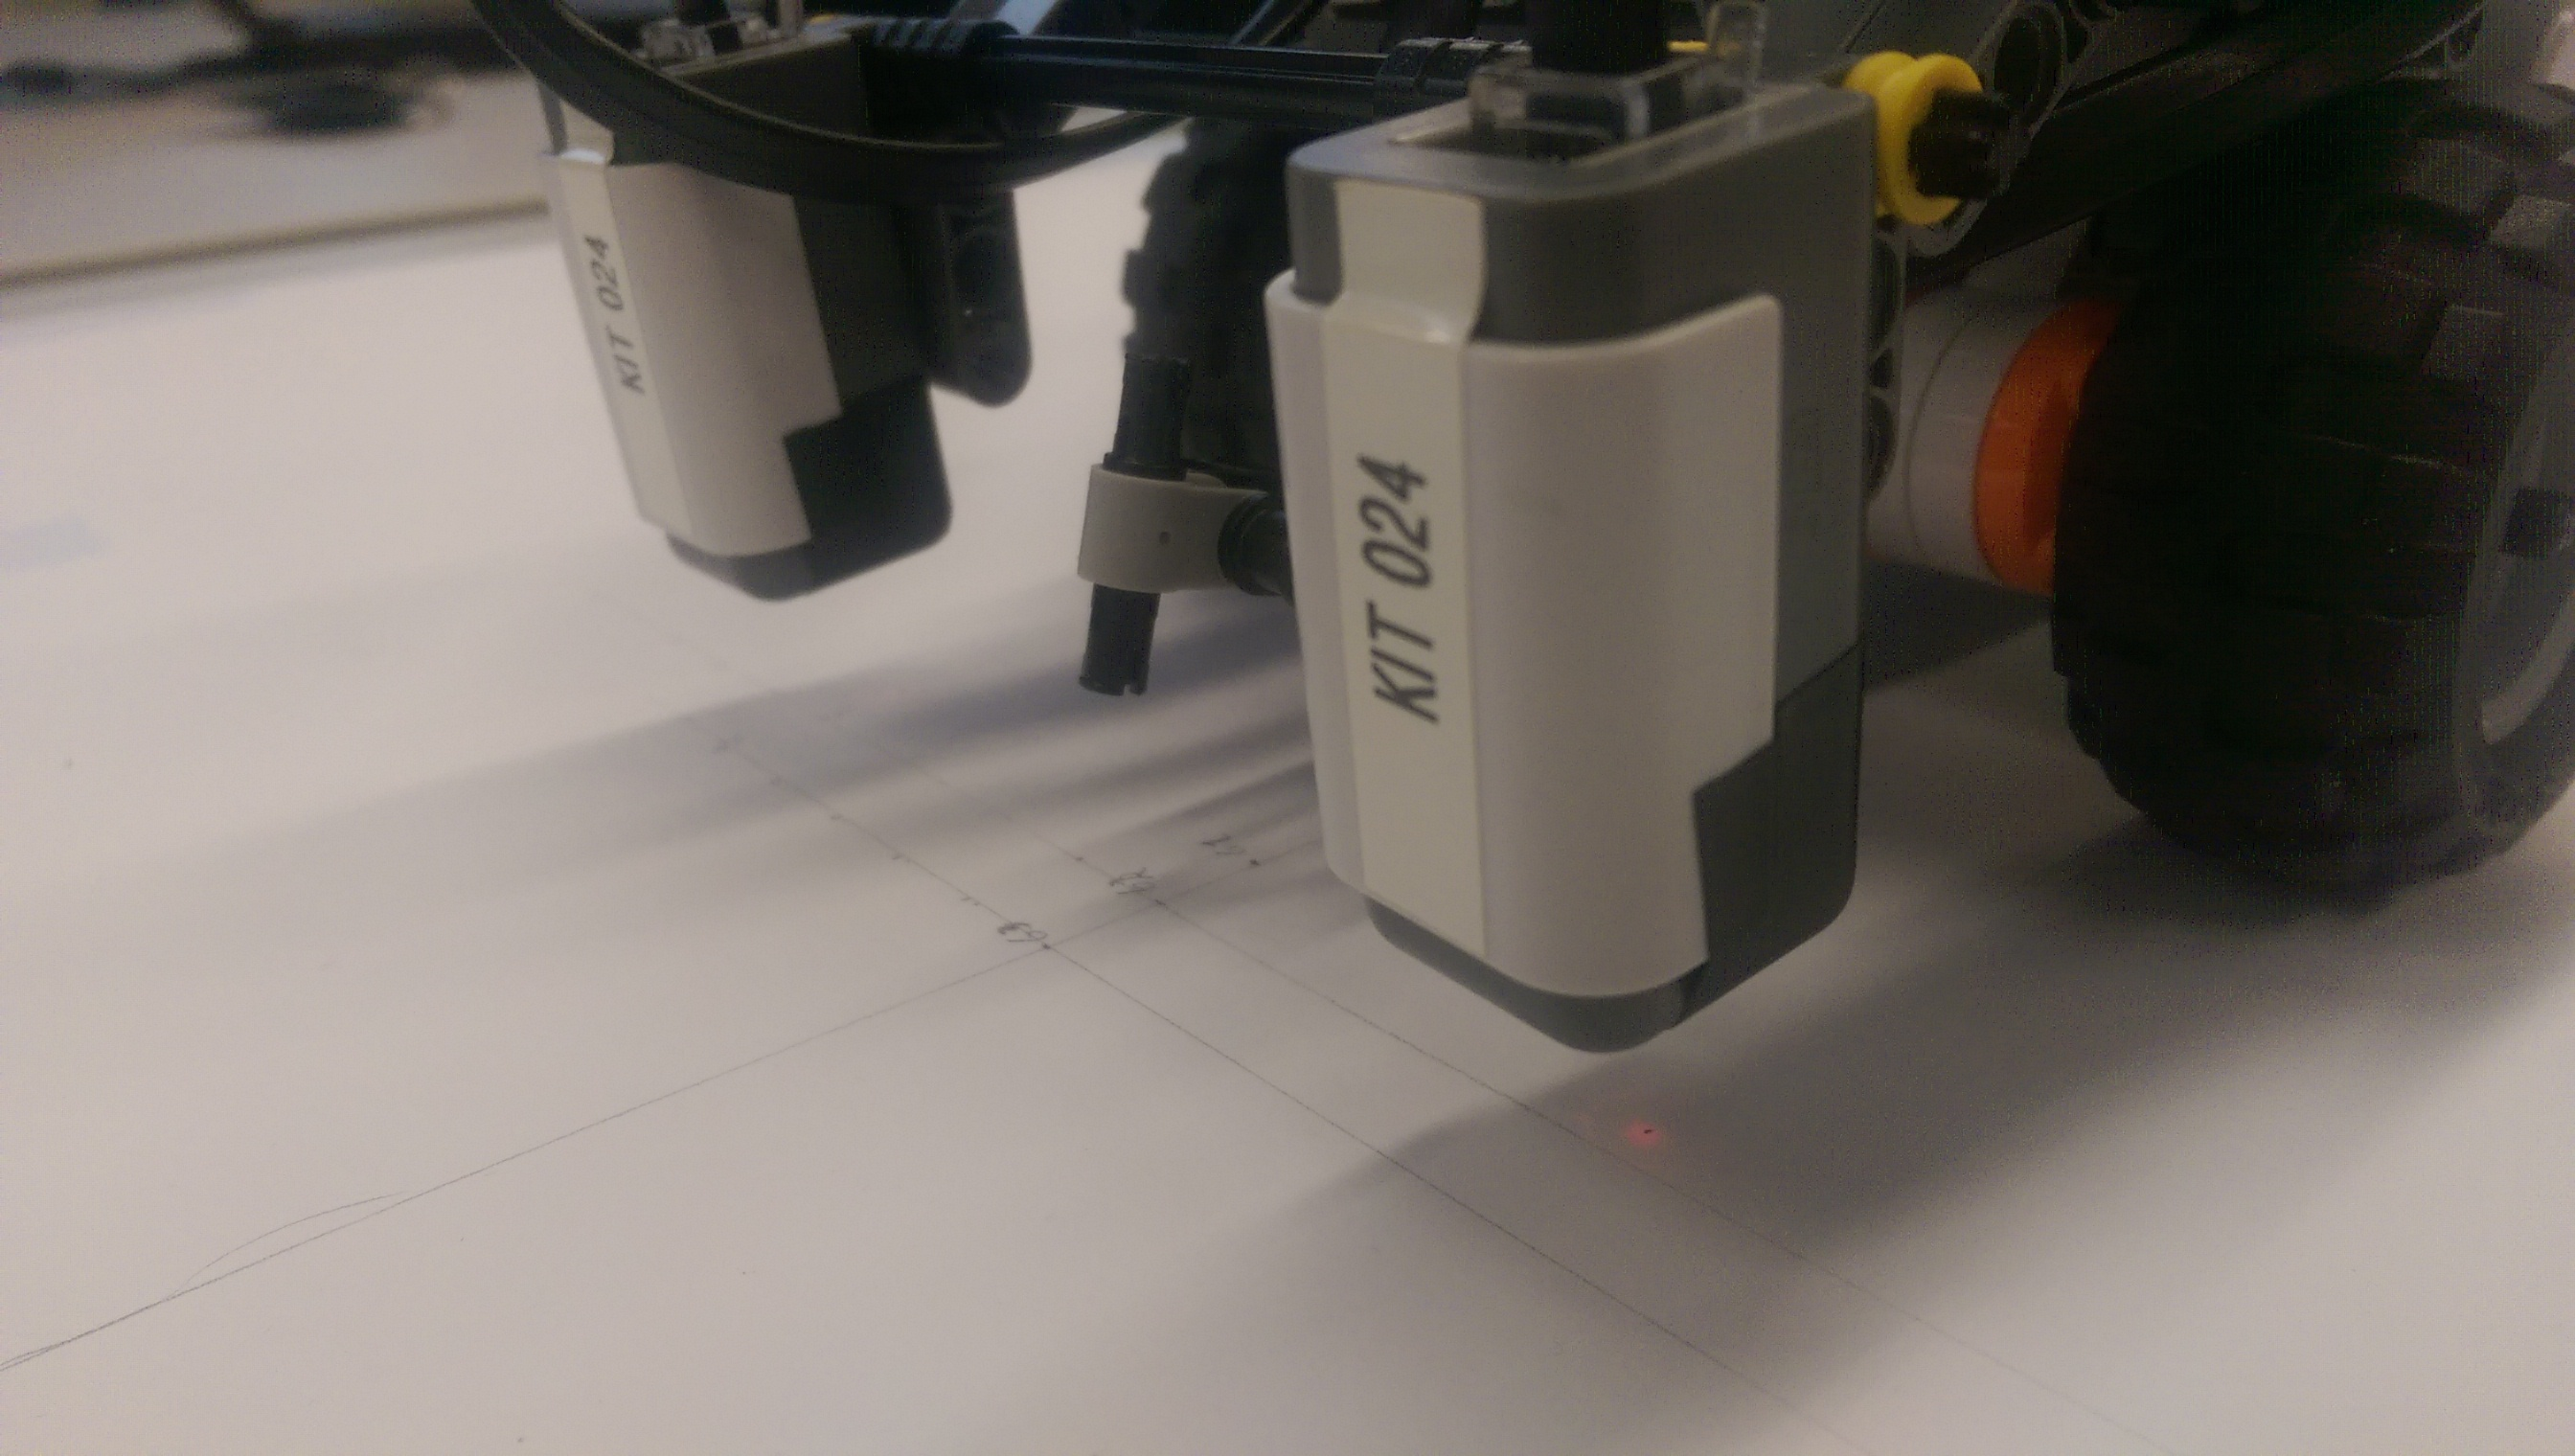
\includegraphics[width=0.8\textwidth]{garage}
\end{figure}


\section{Experimental data processing}

We have obtained 105 pairs of points (see attachment Data.txt). The overall distribution of robot's positions is shown in Fig.\ref{fig:pos} and the overall distribution of robot's heading directions is shown in Fig.\ref{fig:direct}. In Fig. \ref{pics:forward} - \ref{pics:sright} one can see a zoomed distributions of robot's positions and diagrams for distributions of robot's heading directions for all the movement cases. 

\begin{figure}[H]
  \centering
  \caption{Overall distribution of robot's positions.\label{fig:pos}}
  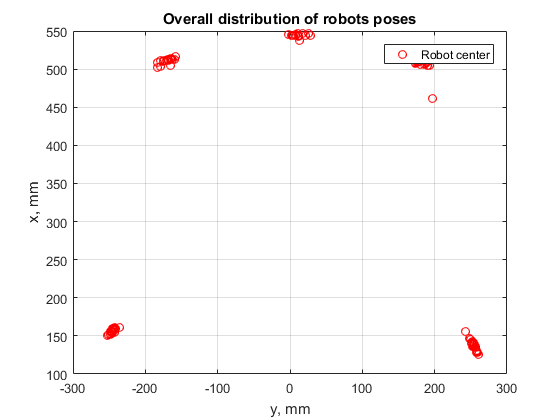
\includegraphics[width=0.6\textwidth]{all}
\end{figure}

\begin{figure}[H]
  \centering
  \caption{Overall distribution of robot's directions.\label{fig:direct}}
  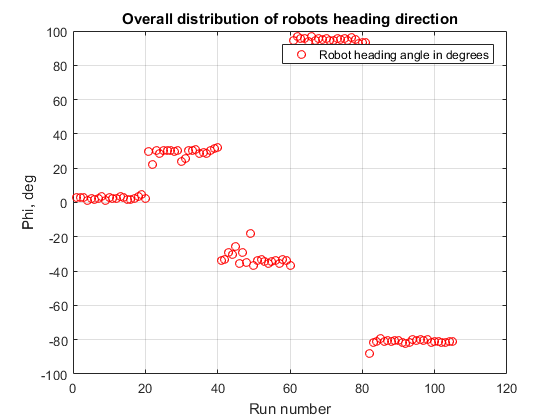
\includegraphics[width=0.6\textwidth]{allphi}
\end{figure}

\begin{figure}[H]
\begin{center}$
\begin{array}{cc}
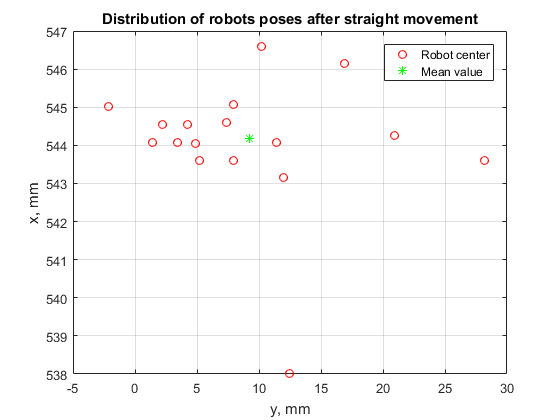
\includegraphics[width=80mm]{s}&
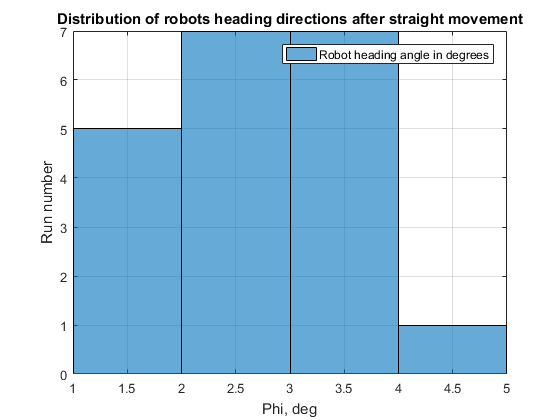
\includegraphics[width=80mm]{sphi}
\end{array}$
\end{center}
\caption{Distribution of the robot's poses and heading directions after forward movement.}
\label{pics:forward}
\end{figure}


\begin{figure}[H]
\begin{center}$
\begin{array}{cc}
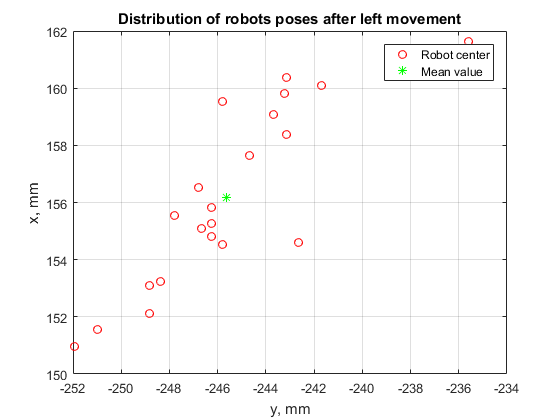
\includegraphics[width=80mm]{LL}&
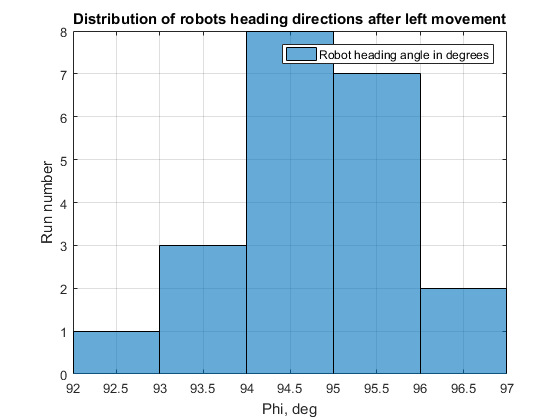
\includegraphics[width=80mm]{LLphi}
\end{array}$
\end{center}
\caption{Distribution of the robot's poses and heading directions after 90$^{\circ}$ left arc movement.}
\label{pics:left}
\end{figure}

\begin{figure}[H]
\begin{center}$
\begin{array}{cc}
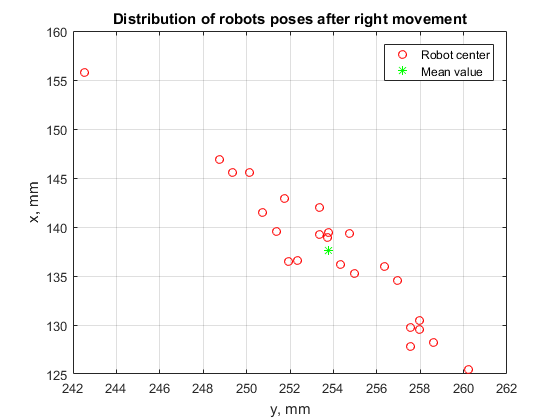
\includegraphics[width=80mm]{RR}&
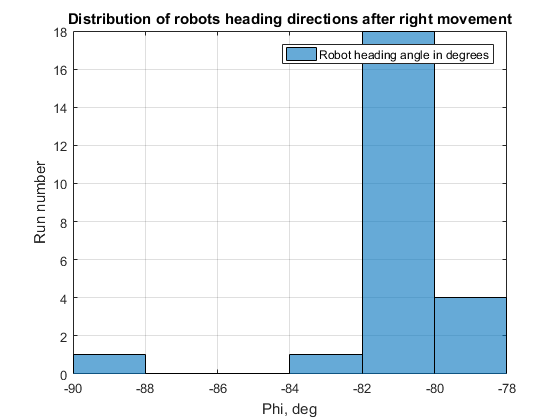
\includegraphics[width=80mm]{RRphi}
\end{array}$
\end{center}
\caption{Distribution of the robot's poses and heading directions after 90$^{\circ}$ right arc movement.}
\label{pics:right}
\end{figure}

\begin{figure}[H]
\begin{center}$
\begin{array}{cc}
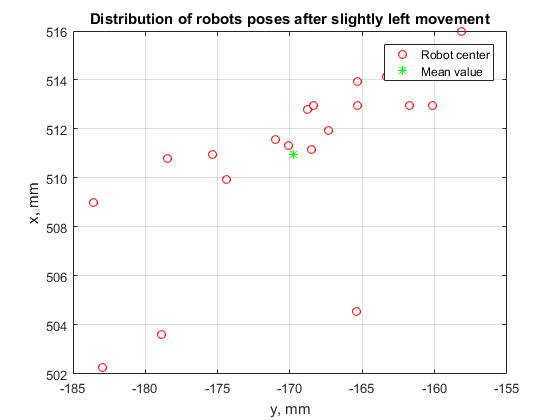
\includegraphics[width=80mm]{l}&
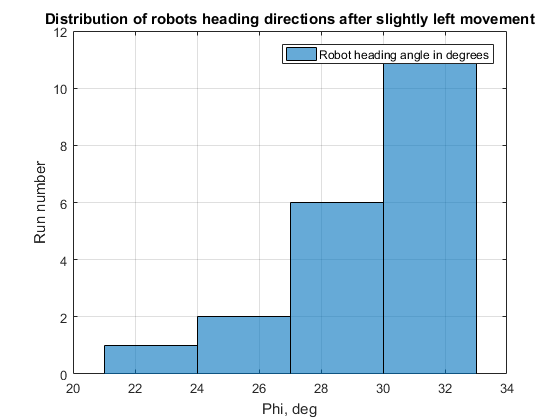
\includegraphics[width=80mm]{lphi}
\end{array}$
\end{center}
\caption{Distribution of the robot's poses and heading directions after 30$^{\circ}$ left arc movement.}
\label{pics:sleft}
\end{figure}

\begin{figure}[H]
\begin{center}$
\begin{array}{cc}
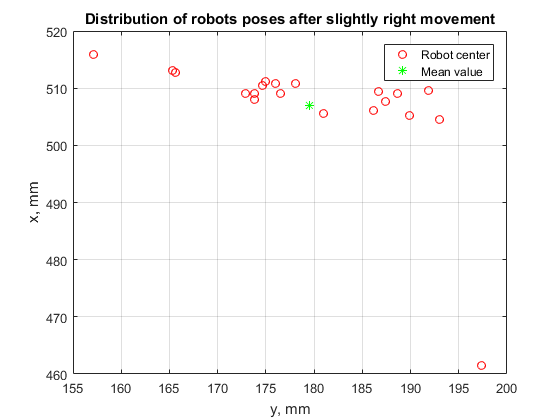
\includegraphics[width=80mm]{r}&
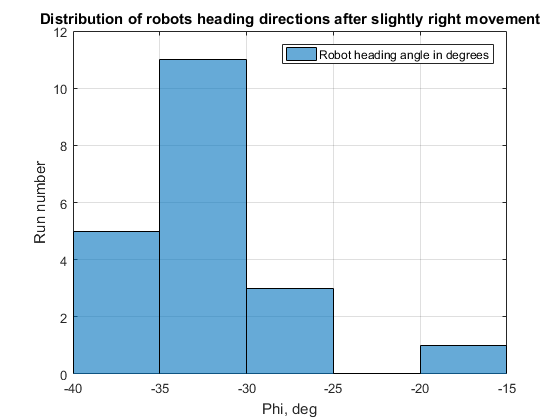
\includegraphics[width=80mm]{rphi}
\end{array}$
\end{center}
\caption{Distribution of the robot's poses and heading directions after 30$^{\circ}$ right arc movement.}
\label{pics:sright}
\end{figure}

For visualization we have used the following matlab code:

\begin{lstlisting}
data = dlmread('Data.txt');

xc = 0.5*(data(:,1)+data(:,3));
yc = 0.5*(data(:,2)+data(:,4));
d = 70;
phi = acos((data(:,4)-data(:,2))./sqrt((data(:,4)-data(:,2)).^2+(data(:,1)-data(:,3)).^2));
phi(41:60) = phi(41:60)-pi;
phi(82:end) = phi(82:end)-pi;

%Overall experiment review

xc = xc - d*cos(phi);
yc = yc + d*sin(phi);
figure(1)
plot(yc,xc,'ro')
grid on
xlabel('y, mm')
ylabel('x, mm')
title('Overall distribution of robots poses')
legend('Robot center')

figure(2)
plot(rad2deg(phi),'ro')
grid on
xlabel('Run number')
ylabel('Phi, deg')
title('Overall distribution of robots heading direction')
legend('Robot heading angle in degrees')

% Forward experiment
figure(3)
plot(yc(1:20),xc(1:20),'ro',mean(yc(1:20)),mean(xc(1:20)),'g*')
mean(yc(1:20))
mean(xc(1:20))
var(yc(1:20))
var(xc(1:20))
grid on
xlabel('y, mm')
ylabel('x, mm')
title('Distribution of robots poses after straight movement')
legend('Robot center','Mean value')

figure(4)
histogram(rad2deg(phi(1:20)))
grid on
ylabel('Run number')
xlabel('Phi, deg')
title('Distribution of robots heading directions after straight movement')
legend('Robot heading angle in degrees')


% Slightly left experiment
figure(5)
plot(yc(21:40),xc(21:40),'ro',mean(yc(21:40)),mean(xc(21:40)),'g*')
mean(yc(21:40))
mean(xc(21:40))
var(yc(21:40))
var(xc(21:40))
grid on
xlabel('y, mm')
ylabel('x, mm')
title('Distribution of robots poses after slightly left movement')
legend('Robot center','Mean value')

figure(6)
histogram(rad2deg(phi(21:40)))
grid on
ylabel('Run number')
xlabel('Phi, deg')
title('Distribution of robots heading directions after slightly left movement')
legend('Robot heading angle in degrees')

% Slightly right experiment
figure(7)
plot(yc(41:60),xc(41:60),'ro',mean(yc(41:60)),mean(xc(41:60)),'g*')
mean(yc(41:60))
mean(xc(41:60))
var(yc(41:60))
var(xc(41:60))
grid on
xlabel('y, mm')
ylabel('x, mm')
title('Distribution of robots poses after slightly right movement')
legend('Robot center','Mean value')

figure(8)
histogram(rad2deg(phi(41:60)))
grid on
ylabel('Run number')
xlabel('Phi, deg')
title('Distribution of robots heading directions after slightly right movement')
legend('Robot heading angle in degrees')

% Left experiment
figure(9)
plot(yc(61:81),xc(61:81),'ro',mean(yc(61:81)),mean(xc(61:81)),'g*')
mean(yc(61:81))
mean(xc(61:81))
var(yc(61:81))
var(xc(61:81))
grid on
xlabel('y, mm')
ylabel('x, mm')
title('Distribution of robots poses after left movement')
legend('Robot center','Mean value')

figure(10)
histogram(rad2deg(phi(61:81)))
grid on
ylabel('Run number')
xlabel('Phi, deg')
title('Distribution of robots heading directions after left movement')
legend('Robot heading angle in degrees')

% Right experiment
figure(11)
plot(yc(82:end),xc(82:end),'ro',mean(yc(82:end)),mean(xc(82:end)),'g*')
mean(yc(82:end))
mean(xc(82:end))
var(yc(82:end))
var(xc(82:end))
grid on
xlabel('y, mm')
ylabel('x, mm')
title('Distribution of robots poses after right movement')
legend('Robot center','Mean value')

figure(12)
histogram(rad2deg(phi(82:end)))
grid on
ylabel('Run number')
xlabel('Phi, deg')
title('Distribution of robots heading directions after right movement')
legend('Robot heading angle in degrees')
\end{lstlisting}

After experimental data was obtained, it should be processed to extract robot position and orientation. 

\begin{figure}[h]
  \centering
  \caption{Base coordinate frame.\label{fig:frame}}
  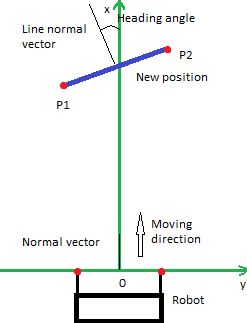
\includegraphics[width=0.4\textwidth]{frame}
\end{figure}

Heading angle of the robot will be calculated as angle between normal vector $(1,0)$ and normal vector to line that goes through points $P_1,P_2.$ It can be calculated using this formulas:

\begin{equation}
\phi = \arccos(\frac{y_2-y_1}{\sqrt{(y_2-y_1)^2+(x_1-x_2)^2}}),
\end{equation}

if robot goes left. And with next one if the robot goes right. This is because $\arccos$ has range $[0, pi]$.

\begin{equation}
\phi = \arccos(\frac{y_2-y_1}{\sqrt{(y_2-y_1)^2+(x_1-x_2)^2}})-\pi.
\end{equation}

After this, robot coordinates can be calculated:

\begin{equation}
X = (\frac{x_1+x_2}{2}-d \cos(\phi),\frac{y_1+y_2}{2}+d \sin(\phi)),
\end{equation}
where $d$ is distance between robot center and point between 2 red dots.

\begin{figure}[h]
  \centering
  \caption{Robot pose calculation\label{fig:frame}}
  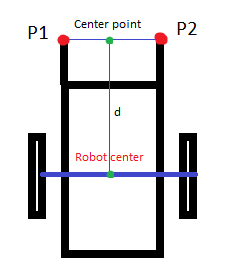
\includegraphics[width=0.4\textwidth]{pose}
\end{figure}
\newpage


After 5 tests, distribution of all poses looks like 5 dense clouds. 


\begin{figure}[h]
  \centering
  \caption{5 clouds of poses.\label{fig:clouds}}
  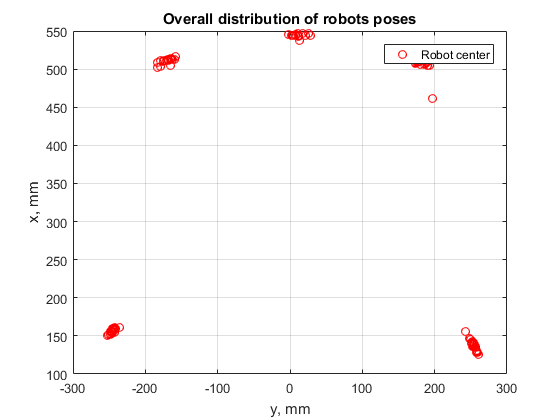
\includegraphics[width=0.6\textwidth]{all}
  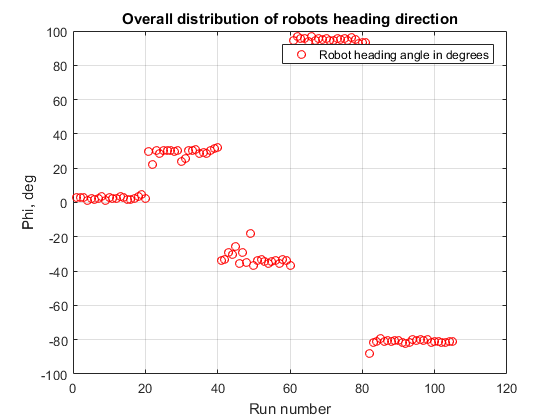
\includegraphics[width=0.6\textwidth]{allphi}
\end{figure}

Now, let's look over each test results.

\newpage
\subsection{Forward movement}
During the forward experiment, the robot was biased to the right. Distribution of positions can be seen on a next figure. Heading direction distribution was shown as a histogram.

\begin{figure}[h]
  \centering
  \caption{Robot positions and heading angle distribution for forward movement test\label{fig:clouds}}
  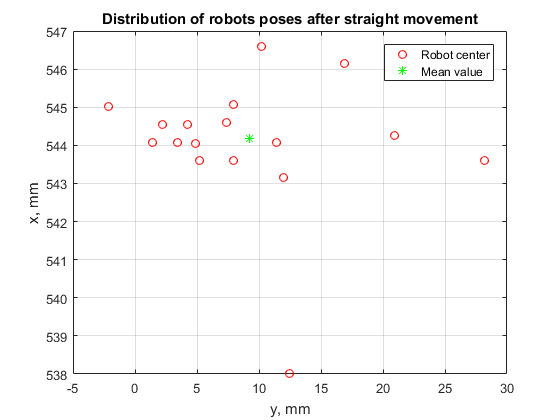
\includegraphics[width=0.6\textwidth]{s}
  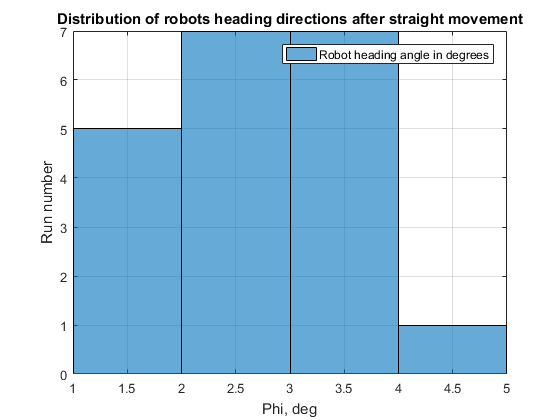
\includegraphics[width=0.6\textwidth]{sphi}
\end{figure}

It can be seen that precision of the reading can be determined by density of the plots and hence by using variance. $var_x = 2.9,var_y = 68.6$. The difference is so big, because the wheels were given the same command.
\newpage
\subsection{Slight left movement}


\begin{figure}[h]
  \centering
  \caption{Robot positions and heading angle distribution for slight left movement test\label{fig:l}}
  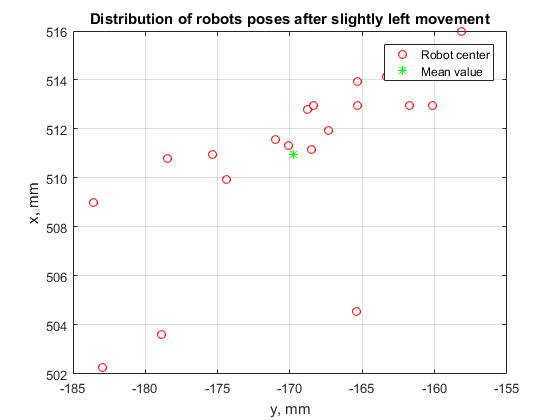
\includegraphics[width=0.6\textwidth]{l}
  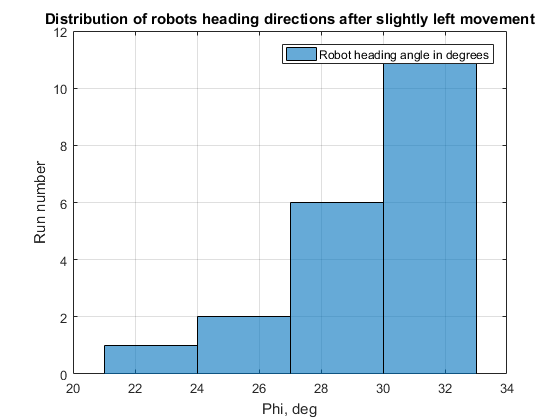
\includegraphics[width=0.6\textwidth]{lphi}
\end{figure}

It can be seen that precision of the reading can be determined by density of the plots and hence by using variance. $var_x = 51.6,var_y = 12.9$
\newpage
\subsection{Slight right movement}


\begin{figure}[h]
  \centering
  \caption{Robot positions and heading angle distribution for slight right movement test\label{fig:r}}
  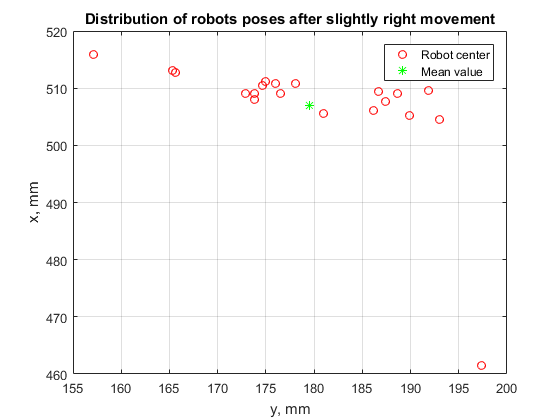
\includegraphics[width=0.6\textwidth]{r}
  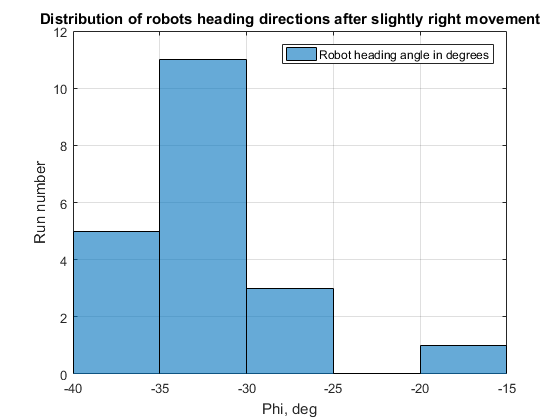
\includegraphics[width=0.6\textwidth]{rphi}
\end{figure}

It can be seen that precision of the reading can be determined by density of the plots and hence by using variance. $var_x = 109,var_y = 122.6$ The variance is so big, because one reading look line an experimental error.
\newpage
\subsection{Left movement}


\begin{figure}[h]
  \centering
  \caption{Robot positions and heading angle distribution for left movement test\label{fig:LL}}
  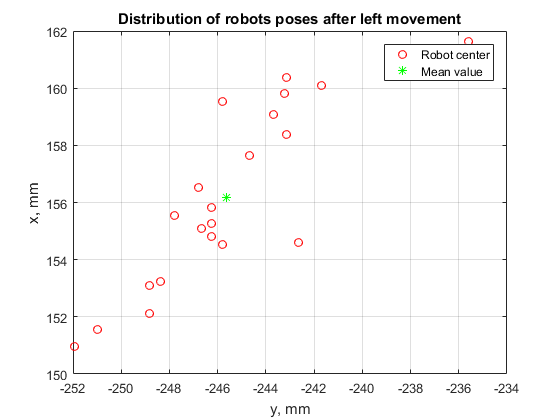
\includegraphics[width=0.6\textwidth]{LL}
  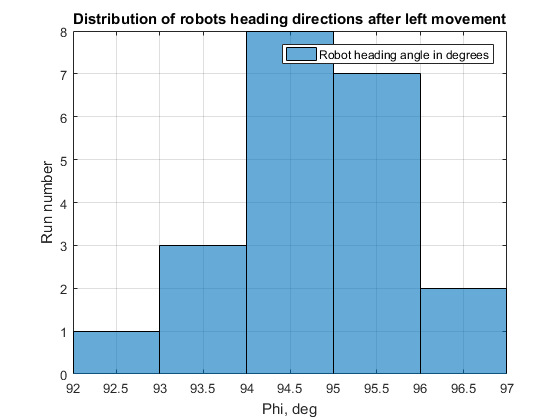
\includegraphics[width=0.6\textwidth]{LLphi}
\end{figure}

It can be seen that precision of the reading can be determined by density of the plots and hence by using variance. $var_x = 9.8,var_y = 12.6$.
\newpage
\subsection{Right movement}


\begin{figure}[h]
  \centering
  \caption{Robot positions and heading angle distribution for right movement test\label{fig:RR}}
  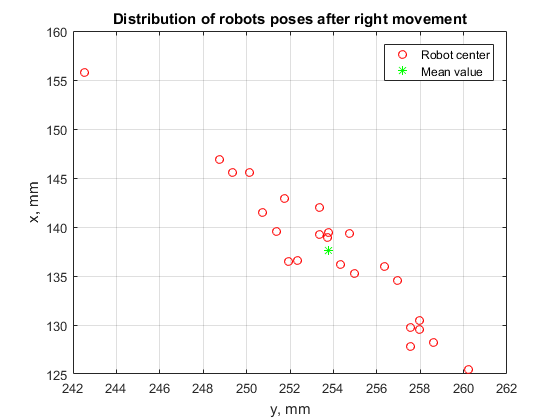
\includegraphics[width=0.6\textwidth]{RR}
  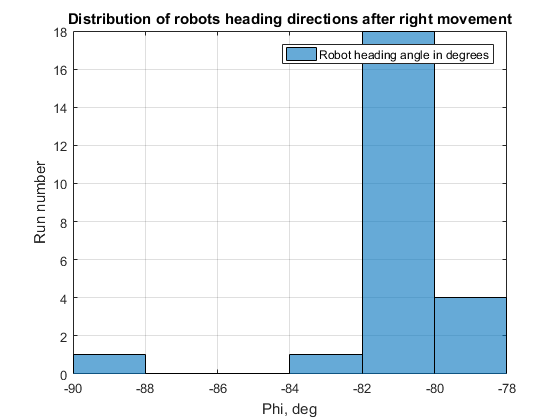
\includegraphics[width=0.6\textwidth]{RRphi}
\end{figure}

It can be seen that precision of the reading can be determined by density of the plots and hence by using variance. $var_x = 50.2,var_y = 15.5$.


\section{Conclusions}
During the experiment we have noticed two new possible error sources. First, we have a flexible caster wheel (Fig), that is impossible to put in the perfectly same position each time we redo the experiment.

//TODO: insert the wheel image

That is an unavoidable error, that can be eliminated only by using a completely different construction of the robot. Second, though the button pressing control is convenient and allow us to install the robot without time limits, the act of pressing can slightly move the robot. However, after several tests on short distances, where the motor error is still not too big, we've concluded that this error is insignificant and cannot be detected by our measurement methods. \\

A precision of the measurement was limited by a precision of a ruler we used. So, each measurement should be taken with $\pm$ 0.05cm.\\
Forward motion was to end in (628, 0) position, 90$^{\circ}$ arc motion to the left -- (-250, 250), 90$^{\circ}$ arc motion to the right -- (250, 250), 30$^{\circ}$ arc motion to the left -- (-160, 600) and 30$^{\circ}$ arc motion to the right -- (-160, 600). The actual positions can be seen in Fig. \ref{pics:forward} - \ref{pics:sright}.


\end{document}
